Design principles:
        \begin{itemize}
            \item there are many of possible paths that cross exactly the same mount of links to go from one node to another
            \item the network can scale easily by changing some parameters
            \item multiple core switches
        \end{itemize}
        
        The main advantage of working with fat trees is that it's optimal interconnect for large-scale clusters, the server are placed at the leafs, switches populate the root and the internal nodes of the tree. This is super regular, all switching elements of a fat-tree are identical.
        It's consist in only one parameter. In fact, given k, you will have have $k$ pods; each pod has two layers; each layer has $\frac{k}{2}$ switches; each switch in the lower layer has connected to $k$ layers; every switch is connected to the aggregation layer. 
        
        Switches and pods are numbered and accessed by an IP address.
        
        There are some open issues
        \begin{itemize}
            \item Workloads
            \begin{itemize}
                \item Small flows (mice flows) requiring low-latency
                \item Large flows (elephant flows) requiring high-throughput
            \end{itemize}
        \end{itemize}
        How we can balance these workloads? Another issue is that TCP does not perform well in data center networks (we have to replace it with for example QUIC or other protocols).
        
        \subsubsection{How to balance traffic flows}
        Let's assume we have many flows from S to D, many equal cost paths going up to the core switches and only one path down from each core switch
        \begin{figure}[h!]
            \centering
            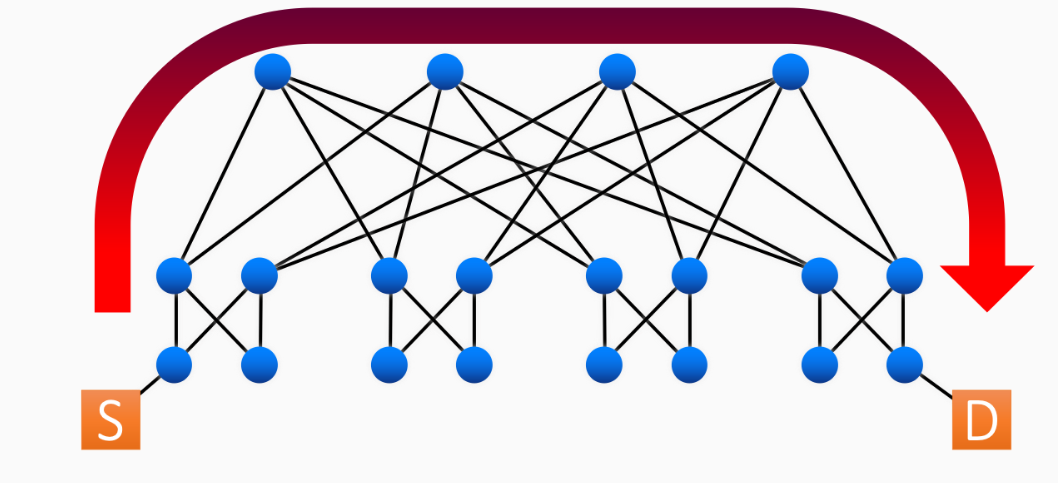
\includegraphics[scale=0.25]{images/trafficflow1.png}
        \end{figure}    
        We can use Equal-Cost Multi-Path routing (ECMP) to balance flow, it randomly allocate paths to flows using hash 0f the flow, but this is agnostic to available resources and can cause long lasting collision between elephant flows.
        
        To avoid this problem we can use Hedera, a technique to detect elephant flows, compute non-conflicting paths and instruct switches to reroute traffic.
    
    \subsection{Networking in virtualized environments}
    We want this because we need the capability to run multiple virtual machines on the same physical host, all the components are created by OS (like switches and bridges).
    \begin{figure}[h!]
        \centering
        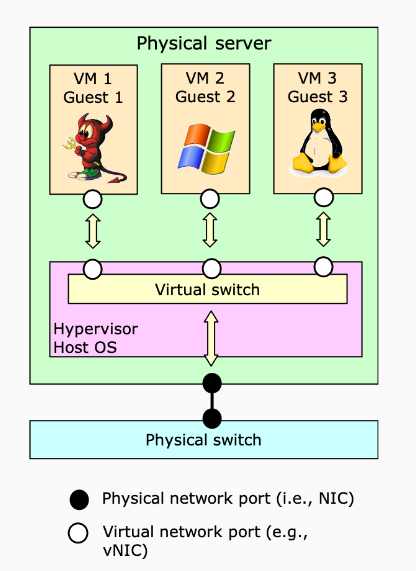
\includegraphics[scale=0.25]{images/virtualnet.png}
    \end{figure}    
    Virtualization introduces additional complexity for networking: we need to deliver traffic from virtual to physical network (and vice versa) and deliver traffic between VMs/LXCs within the same server. We also need to assign IP addresses to VMs/LXCs and provide advanced features such as load balancing, firewall ecc.
    
    In order to do this we need at first to provide Ethernet (L2) connectivity to VMs/containers and then to provide IP connectivity to them.
    
    \subsection{North/South and East/West communications on a single server}
    We can solve the problem presented above with at least three methods
    \begin{itemize}
        \item Virtual switch in the host
        \item In the NIC 
        \item In the external switch
    \end{itemize}   
    \begin{figure}[h!]
        \centering
        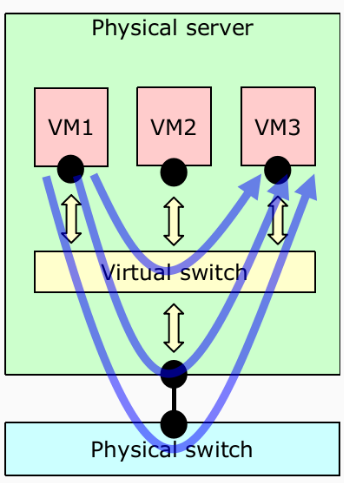
\includegraphics[scale=0.25]{images/virtserver.png}
    \end{figure}
    Historically the first solution (Host-based switching) used was the first one, is the easiest to manage and create. It bring us high bandwidth for inter-VM traffic but it create additional processing overhead and consumes CPU cycles, it require an additional component and it's not clear who controls the switch. This solution it's also called software bridge or softswitch, it uses function given by the kernel to manage packets.
    
    The third one (Hairpin switching) use hardware that is already present (it has to be compatible). It's slower then the previous one but don't use CPU cycles, in any case this solution it's no longer used.
    
    The intermediate solution is the NIC switching (intermediate also in terms of strengths and weaknesses). This solution avoids the problem about who controls edges switches and gave the opportunity to the researcher to innovate the NICs and create the smartNIC\footnote{A NIC with a processor and memory (like a GPU)}.
    
    Host switches is currently the most common solution.
    
    \subsection{Software bridges in Linux}
    A software bridge provide intra-host connectivity to execution containers and handle IP addresses differently from the official IP model (the one IP address per NIC rule). A schema of basic bridging networking in Linux is this:
    \begin{figure}[h!]
        \centering
        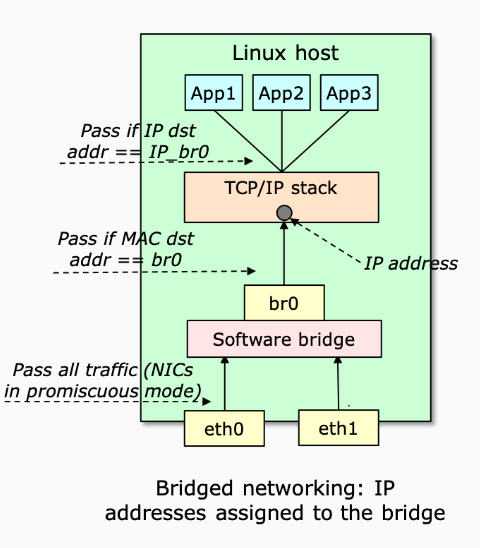
\includegraphics[scale=0.25]{images/bridgeschema.png}
    \end{figure}
    Linux has three main types of software bridges:
    \begin{itemize}
        \item Linuxbridge
        \item macvlan
        \item Open vSwitch
    \end{itemize}
        \subsubsection{Linuxbridge}
        It's the most common and simple one, it behaves like a traditional hardware switch, the NICs has to be in promiscuous mode.
        \subsubsection{Macvlan}
        It's implements a VLAN-like behavior by using MAC addresses instead of tags, it's more like a L2 subinterface derived from the main NIC, each macvlan interface has its own MAC address and can have a distinct IP address. Applications can bind to a specific interface/IP address, it support some mode, the private one makes a VLAN-like behavior, the VEPA mode that allows MAC A to talk with MAC B only if the traffic comes from the external world. And final the bridge mode that macvlan driver act like a bridge.
        
        Linux bridges behaves like a traditional hardware switch the macvlan instead behaves like a bridge, it's simple and fast. So we use macvlan if we need to provide connection to the physical network to your VMs or LXCs. Use bridge if we need to connect VMs or containers on the same host and other cases.
        
        \subsubsection{Open vSwitch}
        Open vSwitch is a software implementation of a virtual multilayer network switch 
    \subsection{Single server: complex services}
    